\documentclass[poster, a1, plainboxedsections]{sciposter}

\usepackage{multicol}
\usepackage{amsmath}
\usepackage{amsfonts}
\usepackage{graphicx}
\usepackage{booktabs}
\usepackage{tikz}
\usepackage{pgfplots}
\usepackage{pgfplotstable} % For importing data from a csv

% Allows us to exclude some bars from certain plots, to allow multicoloured plots
\pgfplotsset{
    discard if/.style 2 args={
        x filter/.code={
            \edef\tempa{\thisrow{#1}}
            \edef\tempb{#2}
            \ifx\tempa\tempb
                \def\pgfmathresult{inf}
            \fi
        }
    },
    discard if not/.style 2 args={
        x filter/.code={
            \edef\tempa{\thisrow{#1}}
            \edef\tempb{#2}
            \ifx\tempa\tempb
            \else
                \def\pgfmathresult{inf}
            \fi
        }
    }
}

%\leftlogo[1.1]{McMaster_BlackLogo.pdf}
\leftlogo[1.1]{eng_logo.png}
\rightlogo[1.1]{STaBLLogoWS.png}
\title{A Software Engineering Capstone Infrastructure that Encourages Spreading
Work Over Time and Team}
\author{Spencer Smith, Christopher Schankula, Lucas Dutton and Christopher Anand}
\institute{Computing and Software Department, McMaster University}
\email{smiths@mcmaster.ca}

\begin{document}

\conference{{\bf CSEE\&T 2025}, IEEE Conference on Software Engineering
Education and Training, Apr 28--29, Ottawa, ON, Canada}

\maketitle

\setlength{\columnseprule}{0pt}
\begin{multicols}{2}

\PARstart {H}{ow} can instructors facilitate spreading out the work in a
software engineering or computer science capstone course across time and among
team members? we propose using a GitHub template that contains all the initial
infrastructure a team needs, including the folder structure, text-based template
documents and template issues. In addition, we propose each team begins the year
by identifying specific quantifiable individual productivity metrics for
monitoring, such as the count of meetings attended, issues closed and number of
commits.

\section{Proposed Infrastructure} \label{SecPropInfrastruc}

\begin{figure}[!h]
\includegraphics[width=1.0\linewidth]{../figures/CourseStructure.drawio.pdf}
\label{FigStructure}
\end{figure}

Github template (link), quantified team charter.

\section{Time Spread Before and After}

Time-Spread Metrics Across Two Classes (T0 on deadline, T2 up to do days prior)

\centering
\begin{tabular}{@{}lrrr@{}}
\toprule
\textbf{Metric}                      & \textbf{2022/23 Value} & \textbf{2023/24 Value} \\ \midrule
Total Commits                        & 6140                        & 5120                        \\
T0 Commits                          & 1471 (23.96\%)              & 942 (18.40\%)               \\
T2 Commits                    & 2377 (38.71\%)              & 1872 (36.56\%)              \\ \bottomrule
\end{tabular}

\begin{figure}[h!]
\centering
\begin{tikzpicture}
\begin{axis}[
    ybar,
    bar width=0.2mm,
    width=0.5\textwidth,
    height=0.35\textwidth,
    symbolic x coords={2022-09-01, 2022-09-02, 2022-09-03, 2022-09-04, 2022-09-05, 2022-09-06, 2022-09-07, 2022-09-08, 2022-09-09, 2022-09-10, 2022-09-11, 2022-09-12, 2022-09-13, 2022-09-14, 2022-09-15, 2022-09-16, 2022-09-17, 2022-09-18, 2022-09-19, 2022-09-20, 2022-09-21, 2022-09-22, 2022-09-23, 2022-09-24, 2022-09-25, 2022-09-26, 2022-09-27, 2022-09-28, 2022-09-29, 2022-09-30, 2022-10-01, 2022-10-02, 2022-10-03, 2022-10-04, 2022-10-05, 2022-10-06, 2022-10-07, 2022-10-08, 2022-10-09, 2022-10-10, 2022-10-11, 2022-10-12, 2022-10-13, 2022-10-14, 2022-10-15, 2022-10-16, 2022-10-17, 2022-10-18, 2022-10-19, 2022-10-20, 2022-10-21, 2022-10-22, 2022-10-23, 2022-10-24, 2022-10-25, 2022-10-26, 2022-10-27, 2022-10-28, 2022-10-29, 2022-10-30, 2022-10-31, 2022-11-01, 2022-11-02, 2022-11-03, 2022-11-04, 2022-11-05, 2022-11-06, 2022-11-07, 2022-11-08, 2022-11-09, 2022-11-10, 2022-11-11, 2022-11-12, 2022-11-13, 2022-11-14, 2022-11-15, 2022-11-16, 2022-11-17, 2022-11-18, 2022-11-19, 2022-11-20, 2022-11-21, 2022-11-22, 2022-11-23, 2022-11-24, 2022-11-25, 2022-11-26, 2022-11-27, 2022-11-28, 2022-11-29, 2022-11-30, 2022-12-01, 2022-12-02, 2022-12-03, 2022-12-04, 2022-12-05, 2022-12-06, 2022-12-07, 2022-12-08, 2022-12-09, 2022-12-10, 2022-12-11, 2022-12-12, 2022-12-13, 2022-12-14, 2022-12-15, 2022-12-16, 2022-12-17, 2022-12-18, 2022-12-19, 2022-12-20, 2022-12-21, 2022-12-22, 2022-12-23, 2022-12-24, 2022-12-25, 2022-12-26, 2022-12-27, 2022-12-28, 2022-12-29, 2022-12-30, 2022-12-31, 2023-01-01, 2023-01-02, 2023-01-03, 2023-01-04, 2023-01-05, 2023-01-06, 2023-01-07, 2023-01-08, 2023-01-09, 2023-01-10, 2023-01-11, 2023-01-12, 2023-01-13, 2023-01-14, 2023-01-15, 2023-01-16, 2023-01-17, 2023-01-18, 2023-01-19, 2023-01-20, 2023-01-21, 2023-01-22, 2023-01-23, 2023-01-24, 2023-01-25, 2023-01-26, 2023-01-27, 2023-01-28, 2023-01-29, 2023-01-30, 2023-01-31, 2023-02-01, 2023-02-02, 2023-02-03, 2023-02-04, 2023-02-05, 2023-02-06, 2023-02-07, 2023-02-08, 2023-02-09, 2023-02-10, 2023-02-11, 2023-02-12, 2023-02-13, 2023-02-14, 2023-02-15, 2023-02-16, 2023-02-17, 2023-02-18, 2023-02-19, 2023-02-20, 2023-02-21, 2023-02-22, 2023-02-23, 2023-02-24, 2023-02-25, 2023-02-26, 2023-02-27, 2023-02-28, 2023-03-01, 2023-03-02, 2023-03-03, 2023-03-04, 2023-03-05, 2023-03-06, 2023-03-07, 2023-03-08, 2023-03-09, 2023-03-10, 2023-03-11, 2023-03-12, 2023-03-13, 2023-03-14, 2023-03-15, 2023-03-16, 2023-03-17, 2023-03-18, 2023-03-19, 2023-03-20, 2023-03-21, 2023-03-22, 2023-03-23, 2023-03-24, 2023-03-25, 2023-03-26, 2023-03-27, 2023-03-28, 2023-03-29, 2023-03-30, 2023-03-31, 2023-04-01, 2023-04-02, 2023-04-03, 2023-04-04, 2023-04-05, 2023-04-06, 2023-04-07, 2023-04-08, 2023-04-09, 2023-04-10, 2023-04-11, 2023-04-12, 2023-04-13, 2023-04-14, 2023-04-15, 2023-04-16, 2023-04-17, 2023-04-18, 2023-04-19, 2023-04-20, 2023-04-21, 2023-04-22, 2023-04-23, 2023-04-24, 2023-04-25, 2023-04-26, 2023-04-27, 2023-04-28, 2023-04-29, 2023-04-30, 2023-05-01},
    xmin=2022-09-01,
    xmax=2023-05-01,
    xtick=\empty,
    nodes near coords = {},
    nodes near coords align={vertical},
    ymin=0,
    ymax=400,
    ylabel={Commits},
    xlabel={Date},
    xlabel style={yshift=5mm},
    legend style={at={(0.5,1)},anchor=north,legend columns=-1},
    ymajorgrids=false,
    grid style=dashed,
]

\addplot [draw=blue,line width=0.01mm, fill=blue!30,discard if not={Highlight}{None}
] table [
    x=Date,
    y=Commits,
    x index=0,col sep=comma
]{../daily_commits_2022-23.csv};

\addplot [draw=red,line width=0.01mm, fill=red!30,discard if not={Highlight}{Red},bar shift=-0.95mm
] table [
    x=Date,
    y=Commits,
    x index=0,col sep=comma
]{../daily_commits_2022-23.csv};

\addplot [draw=orange,line width=0.01mm, fill=orange!30,discard if not={Highlight}{Orange},bar shift=-0.95mm
] table [
    x=Date,
    y=Commits,
    x index=0,col sep=comma
]{../daily_commits_2022-23.csv};
\legend{Normal Day, Due Date, Presentation Date}
\end{axis}
\end{tikzpicture}
\caption{Histogram of Commits for 2022--2023. Dates shown
in red are due dates for major written deliverables, and dates in orange are days where
presentations were scheduled.}\label{Fig_22_23Timeline}
\end{figure}

\begin{figure}[h!]
\centering
\begin{tikzpicture}
\begin{axis}[
    ybar,
    bar width=0.2mm,
    width=0.5\textwidth,
    height=0.35\textwidth,
    symbolic x coords={2023-09-01, 2023-09-02, 2023-09-03, 2023-09-04, 2023-09-05, 2023-09-06, 2023-09-07, 2023-09-08, 2023-09-09, 2023-09-10, 2023-09-11, 2023-09-12, 2023-09-13, 2023-09-14, 2023-09-15, 2023-09-16, 2023-09-17, 2023-09-18, 2023-09-19, 2023-09-20, 2023-09-21, 2023-09-22, 2023-09-23, 2023-09-24, 2023-09-25, 2023-09-26, 2023-09-27, 2023-09-28, 2023-09-29, 2023-09-30, 2023-10-01, 2023-10-02, 2023-10-03, 2023-10-04, 2023-10-05, 2023-10-06, 2023-10-07, 2023-10-08, 2023-10-09, 2023-10-10, 2023-10-11, 2023-10-12, 2023-10-13, 2023-10-14, 2023-10-15, 2023-10-16, 2023-10-17, 2023-10-18, 2023-10-19, 2023-10-20, 2023-10-21, 2023-10-22, 2023-10-23, 2023-10-24, 2023-10-25, 2023-10-26, 2023-10-27, 2023-10-28, 2023-10-29, 2023-10-30, 2023-10-31, 2023-11-01, 2023-11-02, 2023-11-03, 2023-11-04, 2023-11-05, 2023-11-06, 2023-11-07, 2023-11-08, 2023-11-09, 2023-11-10, 2023-11-11, 2023-11-12, 2023-11-13, 2023-11-14, 2023-11-15, 2023-11-16, 2023-11-17, 2023-11-18, 2023-11-19, 2023-11-20, 2023-11-21, 2023-11-22, 2023-11-23, 2023-11-24, 2023-11-25, 2023-11-26, 2023-11-27, 2023-11-28, 2023-11-29, 2023-11-30, 2023-12-01, 2023-12-02, 2023-12-03, 2023-12-04, 2023-12-05, 2023-12-06, 2023-12-07, 2023-12-08, 2023-12-09, 2023-12-10, 2023-12-11, 2023-12-12, 2023-12-13, 2023-12-14, 2023-12-15, 2023-12-16, 2023-12-17, 2023-12-18, 2023-12-19, 2023-12-20, 2023-12-21, 2023-12-22, 2023-12-23, 2023-12-24, 2023-12-25, 2023-12-26, 2023-12-27, 2023-12-28, 2023-12-29, 2023-12-30, 2023-12-31, 2024-01-01, 2024-01-02, 2024-01-03, 2024-01-04, 2024-01-05, 2024-01-06, 2024-01-07, 2024-01-08, 2024-01-09, 2024-01-10, 2024-01-11, 2024-01-12, 2024-01-13, 2024-01-14, 2024-01-15, 2024-01-16, 2024-01-17, 2024-01-18, 2024-01-19, 2024-01-20, 2024-01-21, 2024-01-22, 2024-01-23, 2024-01-24, 2024-01-25, 2024-01-26, 2024-01-27, 2024-01-28, 2024-01-29, 2024-01-30, 2024-01-31, 2024-02-01, 2024-02-02, 2024-02-03, 2024-02-04, 2024-02-05, 2024-02-06, 2024-02-07, 2024-02-08, 2024-02-09, 2024-02-10, 2024-02-11, 2024-02-12, 2024-02-13, 2024-02-14, 2024-02-15, 2024-02-16, 2024-02-17, 2024-02-18, 2024-02-19, 2024-02-20, 2024-02-21, 2024-02-22, 2024-02-23, 2024-02-24, 2024-02-25, 2024-02-26, 2024-02-27, 2024-02-28, 2024-02-29, 2024-03-01, 2024-03-02, 2024-03-03, 2024-03-04, 2024-03-05, 2024-03-06, 2024-03-07, 2024-03-08, 2024-03-09, 2024-03-10, 2024-03-11, 2024-03-12, 2024-03-13, 2024-03-14, 2024-03-15, 2024-03-16, 2024-03-17, 2024-03-18, 2024-03-19, 2024-03-20, 2024-03-21, 2024-03-22, 2024-03-23, 2024-03-24, 2024-03-25, 2024-03-26, 2024-03-27, 2024-03-28, 2024-03-29, 2024-03-30, 2024-03-31, 2024-04-01, 2024-04-02, 2024-04-03, 2024-04-04, 2024-04-05, 2024-04-06, 2024-04-07, 2024-04-08, 2024-04-09, 2024-04-10, 2024-04-11, 2024-04-12, 2024-04-13, 2024-04-14, 2024-04-15, 2024-04-16, 2024-04-17, 2024-04-18, 2024-04-19, 2024-04-20, 2024-04-21, 2024-04-22, 2024-04-23, 2024-04-24, 2024-04-25, 2024-04-26, 2024-04-27, 2024-04-28, 2024-04-29, 2024-04-30, 2024-05-01},
    xmin=2023-09-01,
    xmax=2024-05-01,
    xtick=\empty,
    nodes near coords = {},
    nodes near coords align={vertical},
    ymin=0,
    ymax=325,
    ylabel={Commits},
    xlabel={Date},
    xlabel style={yshift=5mm},
    legend style={at={(0.5,1)},anchor=north,legend columns=-1},
    ymajorgrids=false,
    grid style=dashed,
]

\addplot [draw=blue,line width=0.1mm,fill=blue!30,discard if not={Highlight}{None}
] table [
    x=Date,
    y=Commits,
    x index=0,col sep=comma
]{../daily_commits_2023-24.csv};

\addplot [draw=red,line width=0.1mm,fill=red!30,discard if not={Highlight}{Red},bar shift=-0.95mm
] table [
    x=Date,
    y=Commits,
    x index=0,col sep=comma
]{../daily_commits_2023-24.csv};

\addplot [draw=orange,line width=0.1mm,fill=orange!30,discard if not={Highlight}{Orange},bar shift=-0.95mm
] table [
    x=Date,
    y=Commits,
    x index=0,col sep=comma
]{../daily_commits_2023-24.csv};
\legend{Normal Day, Due Date, Presentation Date}
\end{axis}
\end{tikzpicture}
\caption{Histogram of Commits for 2023--2024. Dates shown
in red are due dates for major written deliverables, and dates in orange are days where
presentations were scheduled.}\label{Fig_23_24Timeline}
\end{figure}

\section*{Team Fairness Before and After}

$$
\text{unfairness}(C) = \frac{ \sum\limits_{c, x \in C, c > x} (c-x)}{(\left|C\right| -
1) \cdot \sum\limits_{c \in C} c}
$$

\noindent where $C$ is the multiset of teammates' numbers of commits to the 
repository.

The index computes the sum of the difference between each teammate's commits
and those who committed less than them, normalized by the number of teammates
(excluding themselves) and the total number of commits. This yields a value
from 0 to 1, called the \textit{unfairness} index, where:

\begin{itemize}
  \item 0 indicates that teammates did an equal amount of work
  \item 1 indicates that all the work was done by one teammate
  \item A value between 0 and 1 indicates the proportion of work 
        per person which could have been given to someone who did less work
\end{itemize}

Fairness is defined as $\text{fairness}(C) = 1 - \text{unfairness}(C)$.

\begin{figure}[h]
\centering
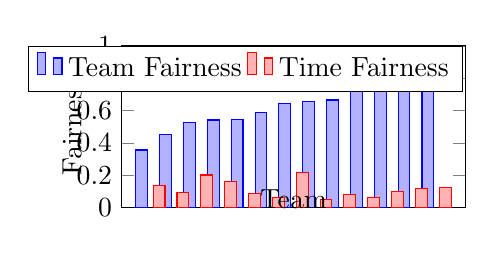
\begin{tikzpicture}
\begin{axis}[
    ybar,
    bar width=1.5mm,
    width=0.49\textwidth,
    height=0.3\textwidth,
    symbolic x coords={Flick-Picker/full-stack, marlon4dashen/Hairesthetics, arkinmodi/project-sayyara, jeff-rey-wang/utrition, mehtaj8/Greenway, Tamas-Leung/CodeChamp, HKanwal/kapstone, paezha/PyERT-BLACK, BillNguyen1999/REVITALIZE, RutheniumVI/UnderTree, agentvv/MTOBridge, NicLobo/Capstone-yoGERT, brandonduong/Farming-Matters},
    xtick=\empty,
    nodes near coords = {},
    nodes near coords align={vertical},
    ymin=0,
    ymax=1,
    ylabel={Fairness},
    ylabel style={yshift=-3mm},
    xlabel={Team},
    xlabel style={yshift=5mm},
    enlarge x limits=0.1,
    legend style={at={(0.36,1)},anchor=north,legend columns=-1},
    ymajorgrids=false,
    grid style=dashed,
]
\addplot coordinates {
    (Flick-Picker/full-stack, 0.3562048588312541)
    (marlon4dashen/Hairesthetics, 0.4509090909090909)
    (arkinmodi/project-sayyara, 0.5239228125826064)
    (jeff-rey-wang/utrition, 0.541871921182266)
    (mehtaj8/Greenway, 0.5447537473233405)
    (Tamas-Leung/CodeChamp, 0.5865051903114187)
    (HKanwal/kapstone, 0.6448184233835252)
    (paezha/PyERT-BLACK, 0.6550335570469799)
    (BillNguyen1999/REVITALIZE, 0.6649842271293376)
    (RutheniumVI/UnderTree, 0.7277227722772277)
    (agentvv/MTOBridge, 0.751219512195122)
    (NicLobo/Capstone-yoGERT, 0.8527835051546392)
    (brandonduong/Farming-Matters, 0.8534278959810875)
};
\addplot coordinates {
    (Flick-Picker/full-stack, 0.13693732643796663)
    (marlon4dashen/Hairesthetics, 0.09129676293855393)
    (arkinmodi/project-sayyara, 0.20175916991791476)
    (jeff-rey-wang/utrition, 0.16419543023821104)
    (mehtaj8/Greenway, 0.086670904852723)
    (Tamas-Leung/CodeChamp, 0.06297005919528731)
    (HKanwal/kapstone, 0.2166401920810488)
    (paezha/PyERT-BLACK, 0.05102825293100133)
    (BillNguyen1999/REVITALIZE, 0.08433884297520666)
    (RutheniumVI/UnderTree, 0.06361620640999799)
    (agentvv/MTOBridge, 0.10007473184455773)
    (NicLobo/Capstone-yoGERT, 0.12032583660750573)
    (brandonduong/Farming-Matters, 0.1269265132901497)
};
\legend{Team Fairness, Time Fairness}
\end{axis}
\end{tikzpicture}
\caption{Fairness of Commits Per Team 2022/23 [n=13; Team Fairness Mean: 0.63, Stddev: 0.15; Time Fairness Mean: 0.12, Stddev: 0.05; Correlation: -0.16]}\label{Fig:Fairness2022/23}
\end{figure}

\begin{figure}[h]
\centering
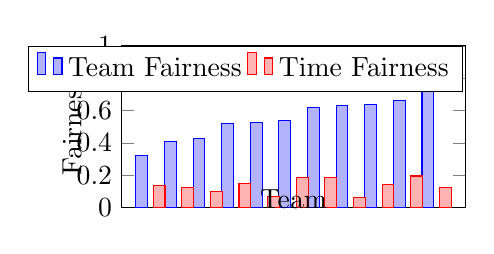
\begin{tikzpicture}
\begin{axis}[
    ybar,
    bar width=1.5mm,
    width=0.49\textwidth,
    height=0.3\textwidth,
    symbolic x coords={r-yeh/grocery-spending-tracker, DangJustin/CapstoneProject, Tusharagg1/chest-x-ray-ai, d-akselrod/SweatSmart, InfiniView-AI/MotionMingle, stanreee/sign-language-learning, RishiVaya/capstone-12, MichaelBreau/nlp-mentalhealth, SammyG7/Mac-AR, beatlepie/4G06CapstoneProjectTeam2, katrina799/4G06CapstoneProjectT5},
    xtick=\empty,
    nodes near coords = {},
    nodes near coords align={vertical},
    ymin=0,
    ymax=1,
    ylabel={Fairness},
    ylabel style={yshift=-3mm},
    xlabel={Team},
    xlabel style={yshift=5mm},
    enlarge x limits=0.1,
    legend style={at={(0.36,1)},anchor=north,legend columns=-1},
    ymajorgrids=false,
    grid style=dashed,
]
\addplot coordinates {
    (r-yeh/grocery-spending-tracker, 0.3200145958766648)
    (DangJustin/CapstoneProject, 0.40943193997856375)
    (Tusharagg1/chest-x-ray-ai, 0.42666666666666664)
    (d-akselrod/SweatSmart, 0.5186666666666666)
    (InfiniView-AI/MotionMingle, 0.525830258302583)
    (stanreee/sign-language-learning, 0.5411013567438148)
    (RishiVaya/capstone-12, 0.6203860480866915)
    (MichaelBreau/nlp-mentalhealth, 0.6298472385428907)
    (SammyG7/Mac-AR, 0.6379532486655624)
    (beatlepie/4G06CapstoneProjectTeam2, 0.6618181818181819)
    (katrina799/4G06CapstoneProjectT5, 0.7661417322834646)
};
\addplot coordinates {
    (r-yeh/grocery-spending-tracker, 0.13841609825545564)
    (DangJustin/CapstoneProject, 0.1259807956104252)
    (Tusharagg1/chest-x-ray-ai, 0.1024815227713779)
    (d-akselrod/SweatSmart, 0.1505020576131687)
    (InfiniView-AI/MotionMingle, 0.07149256677751958)
    (stanreee/sign-language-learning, 0.1860082304526749)
    (RishiVaya/capstone-12, 0.18676949750396077)
    (MichaelBreau/nlp-mentalhealth, 0.06421529443112173)
    (SammyG7/Mac-AR, 0.14521866499267633)
    (beatlepie/4G06CapstoneProjectTeam2, 0.1961316872427984)
    (katrina799/4G06CapstoneProjectT5, 0.12481649941039152)
};
\legend{Team Fairness, Time Fairness}
\end{axis}
\end{tikzpicture}
\caption{Fairness of Commits Per Team 2023/24 [n=11; Team Fairness Mean: 0.55, Stddev: 0.13; Time Fairness Mean: 0.14, Stddev: 0.04; Correlation: 0.15]}\label{Fig:Fairness2023/24}
\end{figure}

\section{Conclusions}

\PARstart {P}{reliminary} data suggests that these steps may have an impact.  In
2022 -- 2023 we observed 24\% of commits happening on the due dates.  After partially
introducing the above ideas in 2023/24, this number improved to 18\%.  To
measure the fairness we introduce a fairness measure based on the disparity
between number of commits between all pairs of teammates.  Going forward we
propose an experiment where commit data and interview data is compared between
teams that use the proposed interventions and those that do not.

\begin{figure}[htbp]
  \centering
  \includegraphics[height=3.2cm,trim={0 0 28.5cm 0},clip]{nserc-logo.jpg}
  \hspace{0.5cm}
  \includegraphics[height=3.2cm,trim={16.5cm 0 0 0},clip]{ontario@2x-print.png}
  \hspace{0.5cm}
  \includegraphics[height=3.2cm,trim={0 0.5cm 0 0.48cm},clip]{outreachlogo.png}  
\end{figure}
  
\end{multicols}

\end{document}